% This is samplepaper.tex, a sample chapter demonstrating the
% LLNCS macro package for Springer Computer Science proceedings;
% Version 2.20 of 2017/10/04
%
\documentclass[runningheads]{llncs}
%
\usepackage{xcolor}
\usepackage{graphicx}
\usepackage{makecell}
\usepackage{textcomp}
%\usepackage{amsmath,amssymb,amsfonts}
\usepackage{algorithm,algorithmic}
\usepackage{wrapfig}
% Used for displaying a sample figure. If possible, figure files should
% be included in EPS format.
%
% If you use the hyperref package, please uncomment the following line
% to display URLs in blue roman font according to Springer's eBook style:
% \renewcommand\UrlFont{\color{blue}\rmfamily}

\renewcommand{\baselinestretch}{0.97}

\begin{document}
%
%\title{Automated Formal Synthesis of Optimal Sizing for Stand-alone Solar Photovoltaic Systems\thanks{Supported by Newton Fund (ref. 261881580) and FAPEAM (Amazonas State Foundation for Research Support, calls 009/2017 and PROTI Pesquisa 2018).}}
\title{Synthesis of Solar Photovoltaic Systems: Optimal Sizing Comparison\thanks{Supported by Newton Fund (ref. 261881580) and FAPEAM (Amazonas State Foundation for Research Support, calls 009/2017 and PROTI Pesquisa 2018).}}
%
%\titlerunning{Abbreviated paper title}
% If the paper title is too long for the running head, you can set
% an abbreviated paper title here
%
\author{Alessandro Trindade\inst{1} \and Lucas Cordeiro\inst{2}} %\orcidID{0000-0001-8262-2919}  \orcidID{0000-0002-6235-4272}
%
\authorrunning{A. Trindade and L. Cordeiro}
% First names are abbreviated in the running head.
% If there are more than two authors, 'et al.' is used.
%
\institute{Federal University of Amazonas, Brazil \email{alessandrotrindade@ufam.edu.br} \and
University of Manchester, UK \email{lucas.cordeiro@manchester.ac.uk}}
\maketitle              % typeset the header of the contribution

\begin{abstract}
The use of formal methods in electrical systems is a new subject, with significant research spanning only the last four years. However, the use of automated synthesis to obtain optimal sizing of solar photovoltaic systems has never been done before. Here our primary goal is to develop and evaluate a sound, automated approach to obtaining optimal sizing of stand-alone photovoltaic systems using program synthesis. We propose a variant of the counterexample guided inductive synthesis (CEGIS) approach, with two phases linking the technical and the cost analysis. First, we synthesize a feasible candidate based on power reliability, which may not attain the lowest cost. Second, the candidate is then verified iteratively with a lower bound cost via symbolic model checking. If the verification step succeeds, the lower bound is adjusted; if it fails, a counterexample provides the optimal solution. Experimental results using seven case studies demonstrate that we can produce an optimal solution within an acceptable run-time. 
%We also present a comparison with a specialized simulation tool over real photovoltaic systems to show the effectiveness of our approach.
%\keywords{Automated verification  \and Model Checking \and Solar photovoltaic systems.}
\end{abstract}

%%%%%%%%%%%%%%%%%%%%%%%%%%%%%%%%%%%%%%%%%%%%%%%%%%%%%%%%
\section{Introduction}
%%%%%%%%%%%%%%%%%%%%%%%%%%%%%%%%%%%%%%%%%%%%%%%%%%%%%%%%
Lack of access to clean and affordable energy is considered a core dimension of poverty~\cite{Hussein2012}. Progress has been made worldwide; in particular, in 2017, the number of people without electricity access fell below $1$ billion threshold for the first time~\cite{IEAweo2018}. In order to provide electricity for all, decentralized systems led by solar photovoltaic (PV) in off-grid and mini-grid systems will be the lowest-cost solution for three-quarters of the additional connections needed~\cite{Hussein2012}. 

In order to simulate or evaluate a PV system, there exist various specialized tools, e.g., RETScreen~\cite{Pradhan} and HOMER~\cite{Swarnkar}; and even general-purpose simulation tools, e.g., MATLAB/Simulink~\cite{Gow1999}. 
 However, these tools are based on simulation; they have the drawback of an incomplete coverage since verification of all possible combinations and potential failures of a system is unfeasible~\cite{ClarkeHV18}. 

Optimization of PV systems is not a recent topic; since the '90s, different techniques using different criteria to find ultimate combinations for design parameters, based on intuitive, numerical, and analytical methods, were proposed and developed~\cite{Alsadi2018}. In $2015$, an automated simulation-based verification technique was applied to verify the correctness of power system protection settings~\cite{Sengupta2015}. In $2017$, a researcher suggested the application of formal methods to verify and control the behavior of computational devices in a smart grid ~\cite{Abate2017}. In $2018$, a verification methodology was applied to PV panels and its distributed power point tracking~\cite{Driouich2018}. In $2019$, an automated verification methodology was proposed to validate stand-alone solar PV systems~\cite{TrindadeCordeiro19}. However, \textit{formal methods and its application to synthesize PV systems are still unexplored in literature}.

Here, we have developed a (non-trivial) variant of counterexample guided inductive synthesis (CEGIS) for synthesizing optimal sizing of stand-alone PV systems using commercial equipment data. Given a correctness specification $\sigma$, our method uses that as a starting point and then iteratively produces a sequence of candidate solutions that satisfy $\sigma$, related to power reliability. In particular, on each iteration, we synthesize the sizing of stand-alone PV systems, but that may not achieve the lowest cost. The candidate solution is then verified via symbolic model checking with a lower bound that serves as the minimum cost of reference; if the verification step does not fail, the lower bound is adjusted. If it fails, then a counterexample is provided with an optimal sizing that meets both power reliability and system cost. Here our focus is not on new criteria or even optimization objectives. Instead, our novelty relies on a practical approach to the pursuit of the optimal solution of PV systems using formal methods. 

Our work makes three significant contributions to advance the state-of-the-art in PV optimal sizing. First, the use of automated symbolic verification in PV systems was uncommon in recent prior studies~\cite{TrindadeCordeiro19}, and specifically, their use in synthesizing PV sizing is novel. Second, we evaluate our approach using different state-of-the-art symbolic verifiers to obtain the best performance in our verification back-end for synthesizing optimal PV systems and compare that to HOMER. Lastly, we discuss the main challenges of applying formal methods to PV systems and also reflect on lessons learned from this practical experience.

%-----------------------------------------------------------
\section{Preliminaries}
\label{sec:AutomatedVerification}
%-----------------------------------------------------------

Fig.~\ref{fig:optimization} illustrates how to obtain the optimal sizing of a stand-alone PV system using the traditional techniques (manual and simulation) and the proposed automated synthesis techniques. Note that the input information is the same for all the methods: weather data, price information, design requirements, as load curve and power demand, and design assumptions. For the automated synthesis, we also define the bound $k$ to restrict the design-space search. On the one hand, if $k$ is too small, then the approach might not return a solution due to the search-space depth. Here we start with a low bound $k$ and incrementally increase it to avoid time and memory constraints on our verification back-end. Therefore, the proper choice of $k$ is essential to this method.
%
\begin{figure}[h]
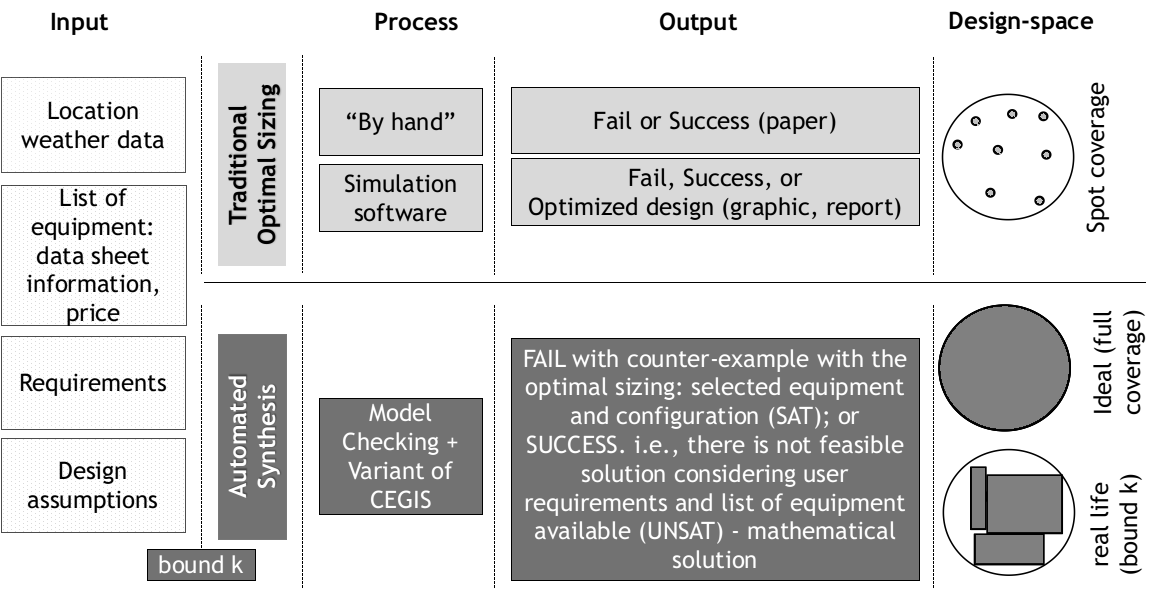
\includegraphics[width=0.8\textwidth]{optimalsizingprocess3}
\centering
\caption{Comparison of optimal sizing methods.}
\label{fig:optimization}
\end{figure}

Both techniques (traditional and automated synthesis)  produce as output either a SUCCESS or FAIL result, thereby considering a feasible technical solution with the lowest cost. On the one hand, when done by simulation, we get a report or graphical result; on the other hand, the automated synthesis technique, which is a mathematical reasoning of a model, presents a counterexample with the optimal solution stored in variables. Furthermore, the design-space coverage during the optimal sizing search is sound and complete when using synthesis.

%-----------------------------------------------------------
\subsection{Program Synthesis}
\label{sec:ProgramSynthesis}
%-----------------------------------------------------------

The basic idea of program synthesis is to automatically construct a program $P$ that satisfies a correctness specification $\sigma$. In particular, program synthesis is automatically performed by engines that use a correctness specification $\sigma$, as starting point, and then incrementally produce a sequence of candidate solutions that partially satisfy $\sigma$~\cite{Abateetal2017}. As a result, a given candidate program $p$ is iteratively refined to match $\sigma$ more closely. Figure~\ref{Counter-Example-Guided-Inductive-Synthesis} illustrates the underlying architecture. 
%
\begin{wrapfigure}{r}{0.5\textwidth}
\begin{center}
%\begin{figure}[h]
%	\centering
	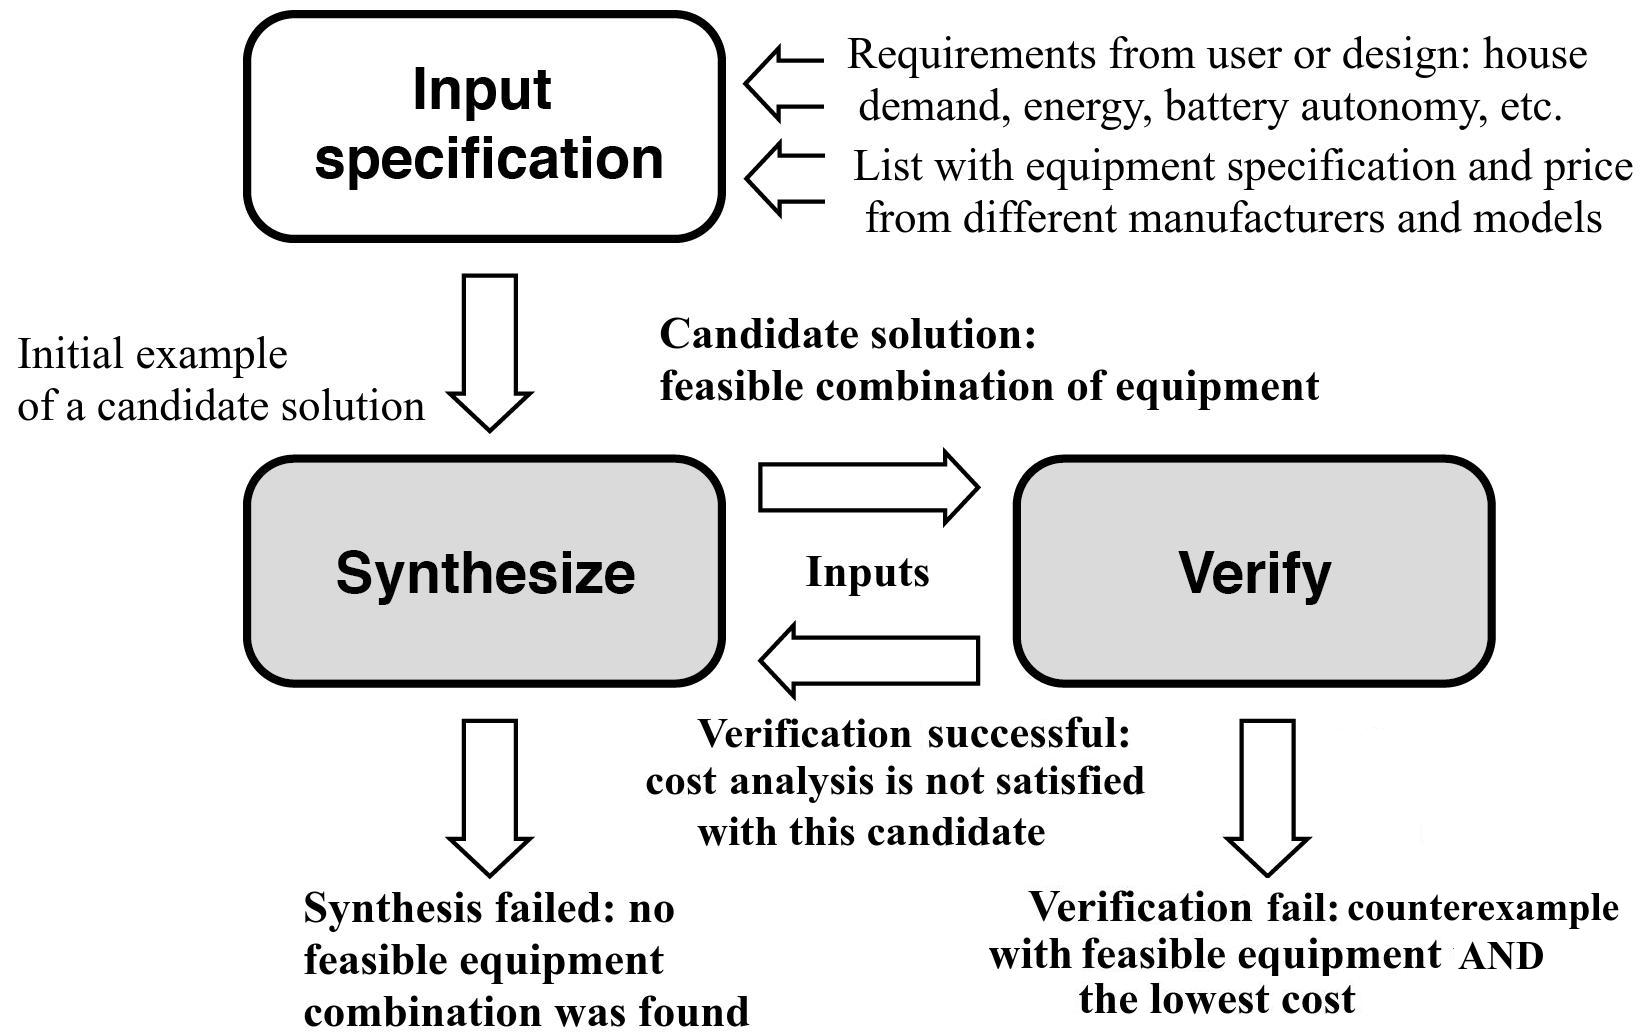
\includegraphics[width=0.5\columnwidth]{fig2_rev2.jpg}
\end{center}	
	\caption{CEGIS in PV system sizing.}
	\label{Counter-Example-Guided-Inductive-Synthesis}
%\end{figure}
\end{wrapfigure}

The correctness specification $\sigma$ provided to our synthesizer is of the form $\exists \vec{F}. \forall \vec{x}. \sigma(\vec{x}, \vec{F})$, where $\vec{F}$ ranges over functions, $\vec{x}$ ranges over ground terms, and $\sigma$ is a quantifier-free (QF) formula typically supported by SMT solvers. The ground terms are interpreted over some finite domain $\mathcal{D}$, where $\mathcal{D}$ can be encoded using the SMT's bit-vectors part. Our specification includes house demand, energy, and battery autonomy; we also provide equipment specifications and prices from different manufacturers and models.

In Figure~\ref{Counter-Example-Guided-Inductive-Synthesis}, regarding traditional CEGIS method, the phases {\sc Synthesize} and {\sc Verify} interact via a finite set of test vectors {\sc inputs}, which is incrementally updated. Given the correctness specification $\sigma$, the {\sc Synthesize} procedure tries to find an existential witness $\vec{F}$ satisfying the specification $\sigma(\vec{x}, \vec{F})$, for all $\vec{x}$ in {\sc inputs} (as opposed to all $\vec{x} \in \mathcal{D}$). If {\sc Synthesize} succeeds in finding a witness~$\vec{F}$, the latter is a candidate solution (i.e., feasible combination of equipment) to the full synthesis formula, which is passed to {\sc Verify} to check whether it is a proper solution ({\it i.e.}, $\vec{F}$ satisfies the specification $\sigma(\vec{x}, \vec{F})$ for all $\vec{x}\in\mathcal{D}$). If this is the case, then the algorithm terminates, i.e., we have found a feasible equipment with the lowest cost; otherwise, in the CEGIS traditional method, additional information is provided to the phase {\sc Synthesize}, in the form of a new counterexample that is added to the {\sc inputs} set and the loop iterates again.

One may notice that each iteration of the traditional CEGIS loop adds a new input to the finite set $INPUTS$, which is then used for synthesis. Given that the full set of inputs $\mathcal{D}$ is finite because we use bit-vector expressions, this means that the refinement loop can only iterate over a finite number of times. However, {\sc Synthesize} may conclude that no candidate solution obeying $\sigma$ for the finite set $INPUTS$ exists, and our synthesis engine can then conclude that no possible equipment combination was found.

In our CEGIS variant, there exist four differences related to the traditional one: 
(1) there exists no test vector and every candidate is generated during the run-time in the {\sc Synthesize} phase and sent to the {\sc Verify} phase; 
(2) if the {\sc Verify} phase is unsuccessful, then a new candidate is generated by {\sc Synthesize} and 
(3) the lower bound of the {\sc Verify} phase is incremented to search for the lowest cost; as a result,
(4) there exists no refinement from the {\sc Verify} phase back to the {\sc Synthesize} phase, i.e., 
a new counterexample is not added to the {\sc input} set since a failure during the {\sc Verify} phase will only discard a given candidate, which could be feasible in the next iteration with a new lower bound.%
%Program synthesis engines that implement the CEGIS approach~\cite{sketch} can automatically produce solutions for a large variety of specifications; 
%here we have used software verifiers based on SMT solvers: CPAChecker~\cite{Beyer2011}, CBMC~\cite{Kroening}, and ESBMC~\cite{esbmc2018}.

%%%%%%%%%%%%%%%%%%%%%%%%%%%%%%%%%%%%%%%%%%%%%%%%%%%%%%%%
\subsection{Sizing Stand-alone Solar PV Systems}
\label{sec:sizing}
%%%%%%%%%%%%%%%%%%%%%%%%%%%%%%%%%%%%%%%%%%%%%%%%%%%%%%%%

A PV system is illustrated in Fig.\ref{fig:blockdiagram}. 
The PV generator, which can be a panel or an array, is a semiconductor device that can convert solar energy into DC electricity. 
For night hours or rainy days, we hold batteries where power can be stored and used. The use of batteries as a storage form implies the presence of a charge controller~\cite{Hansen}. The PV arrays produce DC, and therefore when the PV system contains an AC load, a DC/AC conversion is required. That converter is called inverter; the AC load dictates the behavior of the AC electrical load from the house that will be fed by the system.

\begin{figure}[h]
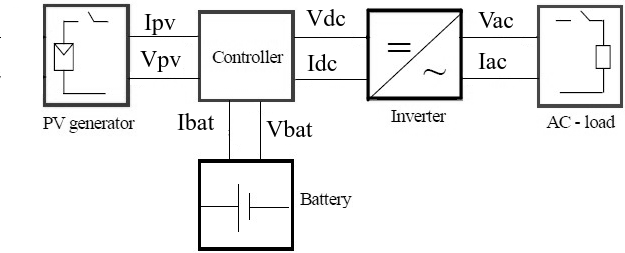
\includegraphics[width=0.7\textwidth]{blockdiagramPVS2_rev}
\centering
\caption{Block diagram for a typical stand-alone PV system~\cite{Hansen}.}
\label{fig:blockdiagram} 
\end{figure}

The sizing check stage will ensure that the system meets the standard project steps related to the critical period solar energy method~\cite{Pinho} and adopting the MPPT (Maximum Power Point Tracking) charge controller, which is the most common one in practice. 
%
Firstly, we need to correct the energy consumption estimated to the load ($E_{consumption}$), which is carried out by Eq.~\ref{eq:Ecorrected}, where the efficiency of batteries ($\eta_{b}$), controller ($\eta_{c}$), and inverter ($\eta_{i}$) are considered~\cite{Pinho} as follows

\begin{equation}
\label{eq:Ecorrected}
E_{corrected} = \frac {E_{consumption}}{\eta_{b} \eta_{c} \eta_{i} }.
\end{equation}

We also need to estimate the energy that can be produced for each panel, called $E_{p}$, in Wh, defined as

\begin{equation}
\label{eq:Ep}
E_{p} = Solar\_Irradiance \times Panel\_Area \times \eta_{p} \times 1000,
\end{equation}

\noindent where the solar irradiance is expressed in terms of $kWh/m^{2}$ and depends on the site where the PV system will be deployed; 
the PV panel area is given in $m^{2}$ and corresponds to the size of one PV panel, and $\eta_{p}$ represents the PV panel efficiency.

The total minimum number of needed solar panels ($N_{TPmin}$) is computed as

\begin{equation}
\label{eq:NTPmin}
N_{TPmin} = \frac{E_{corrected}}{E_{p}}.
\end{equation}

Particularly, the total number of panels in series ($N_{PSmin}$) and parallel ($N_{PPmin}$) are respectively given by

\begin{equation}
\label{eq:NPSmin}
\frac{V_{mppt,min}}{V_{maxPower,TempMax}} \leq N_{PSmin} \leq \frac{V_{mppt,max}}{V_{maxPower,TempMin}},
\end{equation}

\begin{equation}
\label{eq:NPPmin}
N_{PPmin} = \frac{P_{total}}{Number\,Panels\,Series \times P_{max,ref}},
\end{equation}

\noindent where $V_{mppt,max}$ is the maximum operation voltage and $V_{mppt,min}$ is the minimum operation voltage of the charge controller; $V_{maxPower,TempMax}$ and $V_{maxPower,TempMin}$ are the maximum power voltage from the PV module considering the maximum and minimum operational temperature, respectively; $P_{total}$ is the total power demanded from the PV system and $P_{max,ref}$ is the power supplied from one PV panel in $Watts$.
%, $ V_{system} $ is the DC voltage of the bus, normally $12$, $24$ or $48$ V.
%
Regarding batteries, we must first define the total capacity of the battery bank, which can be described as

\begin{equation}
\label{eq:Cbank}
C_{bank} = \frac{E_{corrected} \times autonomy}{V_{system} \times DOD},
\end{equation}

\noindent where the variable $autonomy$ is a design definition; % and normally has a value ranging from $6$ to $48$h; 
$ V_{system} $ is the DC voltage of the bus, and $ DOD $ is the battery deep of discharge (considered of maximum of 25\% here).

Secondly, the total (minimum) number of batteries is computed as 
\begin{equation}
\label{eq:Nbtotal}
N_{B}total = N_{BS}min \times N_{BP}min = \frac{V_{system}}{V_{bat}} \times \frac{C_{bank}}{Battery \, Capacity}.
\end{equation}

Regarding the charge controller, it must initially meet the voltage requirement of the PV system, as described by Eq.~\ref{eq:vcvsystem} to the charge controller voltage: 

\begin{equation}
\label{eq:vcvsystem}
V_{c} = V_{system}.
\end{equation}

The short circuit reference information from the manufacturer's solar panel must be corrected to the cell temperature because the field temperature is higher than the nominal or laboratory temperature, and PV system is temperature dependent, as 

\begin{equation}
\label{eq:iscamb}
I_{sc,amb} = \frac{G}{G_{ref}} \left[I_{sc,ref} +  \mu_{I} \times (T-25) \right]. 
\end{equation}

The controller must meet the maximum current from the PV array given by Eqs. \ref{eq:icmin} and \ref{eq:icicmin} as

\begin{equation}
\label{eq:icmin}
I_{c,min} = I_{sc,amb} \times N_{PP},
\end{equation}

\begin{equation}
\label{eq:icicmin}
I_{c} \geq I_{c,min}.
\end{equation}

The inverter sizing check is performed by means of three equations. Eq.~\ref{eq:vindc} ensures that the input voltage of the controller meets the system voltage. Eq.~\ref{eq:voutac} ensures that the output voltage of the controller meets the AC voltage of the load. Finally, Eq.~\ref{eq:invcheck} ensures that the controller can support the total demand of the load ($Demand$) and the surge power ($P_{surge}$), where $V_{in}DC$ is the nominal input voltage and $V_{out}AC$ is the nominal output voltage of the inverter; $MAX_{AC,ref}$ is the peak power that the inverter can support.

\begin{equation}
\label{eq:vindc} 
V_{in}DC = V_{system}.
\end{equation}

\begin{equation}
\label{eq:voutac} 
V_{out}AC = V_{AC}.
\end{equation}

\begin{equation}
\label{eq:invcheck} 
\left[ (Demand \leq P_{AC,ref}) \, and \, (P_{surge} \leq MAX_{AC,ref}) \right].
\end{equation}

% -------------------------------------------------------
\subsection{Optimal Sizing of PV Systems}
% -------------------------------------------------------
%
The optimal sizing of PV systems is made by the best compromise between two objectives: power reliability and system cost~\cite{Alsadi2018}. 
Regarding power reliability, this work will rely on the critical period solar energy method~\cite{Pinho}, as described in Section~\ref{sec:sizing}. 
Considering the system cost analysis, based on the fact that the deployment location is not specified, our study uses an adapted Life Cycle Cost (LCC) analysis, where only the acquisition cost is considered in the model, i.e., without the operational and maintenance costs~\cite{Alsadi2018}.

%------------------------------------------------------
\section{Synthesizing Optimal Sizing of Stand-alone Solar Photovoltaic Systems}
%Applying Automated Verification to Optimal Sizing of Stand-alone Solar PV Systems}
%------------------------------------------------------
Algorithm~\ref{alg:verification-algorithm} describes our pseudo-code to synthesize stand-alone PV systems using symbolic model checking. 

 \begin{algorithm}
 \caption{Synthesis algorithm}
 \begin{algorithmic}[1]
 \begin{scriptsize}
 \renewcommand{\algorithmicrequire}{\textbf{Input:}}
 \renewcommand{\algorithmicensure}{\textbf{Output:}}
   \REQUIRE weather data (temperature, solar irradiance), list of equipment (datasheet and price information), design requirements (load curve, peak demand, output voltage, battery autonomy), design assumptions (battery state of charge, criteria and objectives for technical and cost analysis).
 \ENSURE FAIL with counter-example showing the optimal sizing; SUCCESS, saying that the project has no feasible solution considering the requirements and the list of equipment available.
  \STATE Initialize variables \\
  \STATE Declare list of PV panels, controllers, batteries, and inverters data and cost \\
%  \STATE Declare list of controllers data and cost \\
%  \STATE Declare list of batteries data and cost \\
%  \STATE Declare list of inverters data and cost \\
  \STATE Declare the maximum possible cost $MaxCost$  \\
  \STATE Declare power demand, power peak, energy consumption \\
  \STATE Declare battery autonomy, depth of discharge, AC voltage \\
  \FOR {$HintCost=0$ to $MaxCost$}
 	\STATE Declare non-deterministic variable to select PV Panel from list \\
 	\STATE Declare non-deterministic variable to select Controller from list \\
 	\STATE Declare non-deterministic variable to select Battery from list \\
 	\STATE Declare non-deterministic variable to select Inverter from list \\ 	
 	\STATE Calculate $E_{corrected}, \, E_{p} $ \\
	\STATE Calculate $N_{TPmin}, \, N_{PSmin}, N_{PPmin} $ \\
 	\STATE Calculate $C_{bank}$ \\
	\STATE Calculate $N_{BS}min, \, N_{BP}min, \, N_{B}total$ \\
	\STATE Requirement enforced by \textbf{assume}$(V_{c})$ \\
 	\STATE Calculate $I_{sc,amb}$ \\
 	\STATE Calculate $I_{c,min}$ \\
 	\STATE Requirement enforced by \textbf{assume}$(I_{c} \wedge V_{in}DC \wedge V_{out}AC)$ \\
%	\STATE Requirement enforced by \textbf{assume}$(V_{in}DC \wedge V_{out}AC )$ \\
%	\STATE Requirement enforced by \textbf{assume}$(V_{out}AC)$ \\
	\STATE Requirement enforced by \textbf{assume}$(Demand \wedge P_{surge})$ \\
%	\STATE Requirement enforced by \textbf{assume}$(P_{surge})$ \\
	\STATE non-deterministic variables hold feasible equipment and cost  \\
	\STATE $F_{obj} \leftarrow  N_{TP}*Panel_{Cost} \, + \, N_{TB}*Battery_{Cost} \, + Controller_{Cost} \, + \, Inverter_{Cost}$ \\
	\STATE Violation check with \textbf{assert}$(F_{obj} > HintCost)$ \\
  \ENDFOR
 \RETURN $(\,)$ 
  \end{scriptsize}
 \end{algorithmic} 
 \label{alg:verification-algorithm}
 \end{algorithm}

Our synthesis algorithm will synthesize constant values; it starts with the input of manufacturers' data and prices of PV panels, batteries, charge controllers, and inverters (Line 2). After that, we define user requirements, i.e., house requirements and design definitions, from Lines 4 and 5. 

The \textit{for}-loop started at Line 6 controls the lowest cost to the PV solution. In particular, it starts with cost $0$ and stops only when the algorithm finds a feasible solution in which the cost breaks the $assertion$ stated in Line 22; if that happens, then our algorithm has found an optimal solution, thereby stating that the {\sc Verify} phase reached a satisfiable condition (\textit{SAT}). The $MaxCost$ value at Line 6 is just a very high value put as a limit to the \textit{for}-loop, that never will be reached because the optimal solution will be found first.

Our synthesis algorithm uses non-deterministic variables to choose one specific constant from a given list of PV panels, controllers, batteries, and inverters (Lines 7 to 10). That procedure ensures that our synthesis engine checks all combinations of items from each equipment, and combine them to assemble a feasible (candidate) PV solution, which meets the user requirements.

Next, we use Eq.~\ref{eq:Ecorrected}, Eq.~\ref{eq:Ep}, Eq.~\ref{eq:NTPmin}, Eq.~\ref{eq:NPSmin}, Eq.~\ref{eq:NPPmin}, Eq.~\ref{eq:Cbank}, Eq.~\ref{eq:Nbtotal}, Eq.~\ref{eq:iscamb}, and Eq.~\ref{eq:icmin} to calculate the sizing variables (Lines 11 to 17). The directive \textit{assume} (Lines 15, 18 and 19) ensures the compatibility of the chosen items from the list of equipment: the {\sc Verify} phase uses only the item (among all the possible ones) that satisfies the statements of Lines 15, 18 and 19. Therefore, our synthesis algorithm reaches Line 20 with one feasible solution, and the cost of that solution is calculated in $F_{obj}$ (Line 21). 

If our algorithm does not find a feasible solution among the item of equipment that was provided to our {\sc Synthesize} phase, then the result is an unsatisfiable (\textit{UNSAT}), i.e., the program finishes and does not find a solution. It indicates that it was not possible to combine the items of each equipment and create a feasible solution. The main challenge for the {\sc Synthesize} phase is to find a feasible candidate solution regarding the constraints and user requirements. Related to our {\sc Verify} phase, the challenge is to find the lowest acquisition cost from a list of equipment and components that are provided from the {\sc Synthesize} phase. 
Note that the process described here in completely automated and that a validation is performed by our {\sc Verify} phase to ensure that the approach is sound.

%---------------------------------------------------------------------------
\section{Results and Discussion}
%---------------------------------------------------------------------------

\textbf{Case studies.} We have performed seven case studies to evaluate our proposed synthesis approach, as described in the first column of Table~\ref{tab1} 
(\textit{Specification}). These case studies were defined based on the usual electrical load found in riverside communities of the Amazon State in Brazil~\cite{Agrener2013,TrindadeCordeiro19}. Except for case 7, which was idealized as a small-town solution to support few lamps and a 12k BTUs air-conditioner. For all cases, an estimated load curve (kWh) was defined based on the electronics consumers in each house.

Our synthesis algorithm was fed with data and costs of forty equipment items from ten different manufacturers of PV systems. Furthermore, three start-of-art verification tools, CBMC,\footnote{Command-line: \$ cbmc -\phantom{}-unwind 100 filename.c -\phantom{}-trace} ESBMC,\footnote{Command-line: \$ esbmc filename.c -\phantom{}-no-bounds-check -\phantom{}-no-pointer-check -\phantom{}-unwind 100 -\phantom{}-boolector} and CPAchecker,\footnote{Command-line: \$ scripts/cpa.sh -heap 64000m -config config/bmc-incremental.properties -spec config/specification/sv-comp-reachability.spc filename.c} were used as our verification engine to compare our approach effectiveness and efficiency. It is important to mention that ESBMC with Z3 solver (version 4.7.1) in ``incremental mode'' was tested as well to reduce memory consumption; however, it was reported an ``internal failure'' error message. %caused by a bug in the solver that was not solved until the end of the tests.

\noindent \textbf{Simulation Tool and Assumptions.} Related to off-the-shelf simulation tools, only HOMER Pro performs off-grid system with battery backup analysis and includes economical analysis. Therefore, in this study, HOMER Pro will be the simulation tool used to comparison. HOMER Pro:

%\textcolor{red}{reescrevi os itens todos, para tornar a leitura mais tranquila}
\begin{itemize}
\item is available only for Microsoft Windows and its annual standard subscription costs US\$ $504.00$~\cite{HOMER}; 
\item it does not have LCC cost in its reports, only Net Present Cost (NPC). But it was possible to obtain LCC from NPC; 
\item the optimization analysis of HOMER allows us to define a load curve and temperature according to data collected from online databases. However, in order to allow a correct comparison, the curve load and the temperature were defined the same as automated synthesis tools; 
\item it does not have a explicit equipment called a charge controller. During the tests, it was chosen the ``load-following'' option which produces only enough power to meet the demand~\cite{HOMER} and (usually) presents a not overestimated solution; 
\item it was assumed the value of 95\% for the availability of the PV system. By definition, 'availability' is the percentage of time at which a power system is capable of feed the load requirements~\cite{Khatib2014}. For ordinary house electrical load, 95\% is considered acceptable;
\item it was assumed a string of two batteries in order to match the voltage of the system of $24$ V DC that was used for the automated synthesis tool; 
\item it was included a generic flat-plate PV of $1$ kW and generic lead-acid batteries of $1$ kW as well (and with capacity of $83.4$ Ah according to HOMER Pro modeling). HOMER, during run-time, decides the size in kW of each module, based on feasibility and lower cost.
\end{itemize}

\noindent \textbf{Setup.} All experiments regarding the verification tools were conducted on an otherwise idle Intel Xeon CPU E5-4617 ($8$-cores) with $2.90$ GHz and $64$ GB of RAM, running Ubuntu $16.04$ LTS $64$-bits. For HOMER Pro, it was used an Intel Core i5-$4210$ ($4$-cores), with $1.7$ GHz and $4$ GB of RAM, running Windows 10. The experiments were performed with a predefined time out of $240$ minutes.

\noindent \textbf{Objectives.} Our evaluation aims to answer three experimental questions: 
\textit{EQ1} \textbf{(soundness)} Does our automated synthesis approach provide correct results?, 
\textit{EQ2} \textbf{(performance)} How do the software verifiers compare to each other?, and 
\textit{EQ3} \textbf{(state-of-the-art)} how does our formal synthesis tool compare to a specialized simulation tool?

\noindent \textbf{Results.} CPAchecker was able to synthesize the optimal sizing in six out of seven case studies (cases $1$ to $6$): the result was produced within the time limit, which varied from $134.71$ to $235.75$ minutes. 
Only case study $7$ led to a \textit{time out} result in CPAchecker, i.e., it was not solved within $240$ minutes.
The violation (SAT result) indicated in Table~\ref{tab1} 
is the $assert$ of line $22$ from Algorithm~\ref{alg:verification-algorithm}. CBMC and ESBMC are unable to produce any conclusive result. Situations of \textit{time out} or \textit{out of memory} occurred; this partially answers the \textit{EQ2} and \textit{EQ3}. 

HOMER Pro was able to evaluate six case studies (cases $1$, $2$, $4$, $5$, $6$, and $7$), and within a time shorter than $30$ seconds, which was much faster than the proposed automated synthesis tool (cf.~\textit{EQ2}). Case study $3$ was not possible to be simulated since HOMER Pro does not have the feature of adjusting the battery autonomy, i.e., the tool always tries to feed with electricity the given load during $365$ days/year. 

Comparing the results between the formal synthesis with CPAchecker and HOMER Pro, it was observed that most results are quite similar, in terms of technical solution and cost (cf. Table~\ref{tab1}). Mainly related to LCC, the cost was very close in cases $1$, $4$, $5$ and $6$, with difference varying from $0.23$\% to $17.4$\%. Even adopting the same price per kW to the PV panels, inverters, and batteries, HOMER Pro does not use costs related to charge controllers, which were introduced into the CPAchecker modeling. The premise used in CPAchecker to adopt a fixed annual cost for operation and maintenance can produce some impact as well at this discrepancy; however, it is not significant since this annual cost is too small when compared to the resulting LCC value. However, there exists a vast divergence in case study $2$, where the costs presented by HOMER Pro were $54$\% higher than the automated synthesis tool, probably because of the operation and maintenance costs assumed by the automated synthesis tool were underestimated to that specific load. 

In general, the size of the PV panels and battery bank were larger in HOMER Pro than with our formal synthesis approach. To compare the results obtained from the optimization, the authors have four PV systems deployed and monitored since June $2018$ in a riverside community in the Amazonas State, Brazil, with similar demands presented by case studies $1$, $4$, $5$, and $6$, with a configuration of $3$ $\times$ $325$ W ($3$S) panels and $4$ $\times$ $220$ Ah ($2$S-$2$P $= 440$ Ah) lead-acid batteries. These deployed systems are closer to the result presented by the proposed formal synthesis approach than HOMER Pro, thereby showing that the solution is sound, which answers \textit{EQ1}.

For the inverters, HOMER Pro suggests a value in kW very close to the peak of every case study, and it is just a reference value and not a commercial value of the employed inverter. The proposed synthesis tool, however, presents inverters that are commercial and can be found off-the-shelf. Therefore is a PRO to the formal synthesis method.

Concerning to charge controllers, as it was reported in this section, HOMER Pro does not include it as an explicit equipment in its mathematical model, only the synthesis tool presents a commercial controller and includes it during the cost analysis. Therefore, the formal synthesis method presents more reliable results than HOMER Pro.

Case study $7$ was not solved by the synthesis tool within the time limit established during the experimental phase. Case study $3$ was not possible to simulate in HOMER Pro, because its restriction does not allow one to set the battery autonomy, thus resting both without parameters to comparison.

\noindent \textbf{Threats to validity.} We have reported a favorable assessment of the proposed method. Nevertheless, we have also identified four threats to the validity of our results that can be further assessed and constitute future work: (1) improvement of the power reliability analysis: to include loss of load probability or loss of power supply probability, which can make the analysis more accurate; (2) improvement of the system cost analysis by including operational and maintenance costs to the adopted LCC analysis; (3) to increase the equipment and manufacturers database: this will increase the complexity of the optimization, but the result will also allow improved sizing; and (4) to compare the results of our approach with an off-the-shelf PV sizing/optimization software: this will validate the results obtained, and it allows a simulation-verification comparison.

\noindent \textbf{Conclusion.} Summarizing, our synthesis tool is capable of presenting a solution, which is far detailed and close to the commercial reality than the solution presented by HOMER Pro. In particular, our automated synthesis method can provide all the details of every component of a PV system solution, with complete electrical details from datasheet of manufacturers, including the model of the component, nominal current, and voltage. In this respect, even the manufacturer's brand can be presented (in Table~\ref{tab1} it was removed to avoid some advertising).
%
%used with the SMT incremental mode\footnote{Command-line: \$ esbmc filename.c -\phantom{}-no-bounds-check -\phantom{}-no-pointer-check -\phantom{}-unwind 100 -\phantom{}-smt-during-symex -\phantom{}-smt-symex-guard -\phantom{}-z3} enabled with the goal of reducing memory usage; we have also used the SMT solver Z3 version 4.7.1~\cite{DeMoura}.

\begin{table}[!t]
\caption{Case studies and results: optimization of PV systems \textcolor{red}{could you please remove the columns for CBMC and ESBMC and just mention in the paper that both verifiers produce MO and TO, respectively?}.}\label{tab1}
\begin{tabular}{|c|c|c|c|c|}
\hline
\hline
Tools & \makecell{CPAchecker 1.8\\(MathSAT 5.5.3)}& \makecell{CBMC 5.11\\(MiniSat 2.2.1)} & \makecell {ESBMC 6.0.0\\(Boolector 3.0.1)} & HOMER Pro 3.13.1\\
\hline
\hline
Specification & Result & Result & Result & Result \\
\hline
\makecell{\textbf{Case Study 1}\\Peak:342W\\Surge:342W \\E:3,900Wh/day\\Autonomy:48h} & \makecell{SAT (172.03 min) \\NTP:1$\times$340W (1S)\\NBT:8$\times$105Ah (2S-4P)\\Controller 15A/75V\\Inverter 700W/48V\\LCC: US\$ 7,790.53} & OM & TO & \makecell{(Time: 0.33 min)\\2.53 kW of PV\\NBT:12$\times$83.4Ah (2S-6P)\\0.351kW inverter\\LCC: US\$ 7,808.04}\\
\hline
\makecell{\textbf{Case Study 2}\\Peak:814W\\Surge:980W\\E:4,880Wh/day\\Autonomy:48h} & \makecell {SAT (228.7 min) \\NTP:2$\times$330W (2S)\\NBT:10$\times$105Ah (2S-5P)\\Controller 20A/100V DC\\Inverter 1,200W/24V \\LCC: US\$ 8,335.90} & OM & TO & \makecell{(Time: 0.18 min)\\3.71 kW of PV\\NBT:20$\times$83.4Ah (2S-10P)\\0.817kW inverter\\LCC: US\$ 12,861.75} \\
\hline
\makecell{\textbf{Case Study 3}\\Peak:815W\\Surge:980W\\E:4,880Wh/day\\Autonomy:12h} & \makecell {SAT (166.13 min) \\NTP:4$\times$150W (4S)\\NBT:4$\times$80Ah (2S-2P)\\Controller 15A/100V DC\\Inverter 1,200W/24V \\LCC: US\$ 7,306.27} & OM & TO & Not possible \\
\hline
\makecell{\textbf{Case Study 4}\\Peak:253W\\Surge:722W\\E:3,600Wh/day\\Autonomy:48h} &  \makecell {SAT (143.71 min) \\NTP:4$\times$150W (4S)\\NBT:10$\times$80Ah (2S-5P)\\Controller 15A/75V\\Inverter 750W/24V \\LCC: US\$ 7,816.31} & OM & TO & \makecell{(Time: 0.23 min)\\2.42 kW of PV\\NBT:12$\times$83.4Ah (2S-6P)\\0.254kW inverter\\LCC: US\$ 7,677.95}\\
\hline
\makecell{\textbf{Case Study 5}\\Peak:263W\\Surge:732W\\E:2,500Wh/day\\Autonomy:48h} &  \makecell {SAT (134.93 min) \\NTP:1$\times$340W (1S)\\NBT:6$\times$105Ah (2S-3P)\\Controller 15A/75V\\Inverter 400W/24V \\LCC: US\$ 7,252.14} & OM & TO & \makecell{(Time: 0.18 min)\\1.59 kW of PV\\NBT:10$\times$83.4Ah (2S-5P)\\0.268kW inverter\\LCC: US\$ 6,175.57} \\
\hline
\makecell{\textbf{Case Study 6}\\Peak:322W\\Surge:896W\\E:4,300Wh/day\\Autonomy:48h} &  \makecell {SAT (235.75 min) \\NTP:2$\times$200W (2S)\\NBT:10$\times$105Ah (2S-5P)\\Controller 15A/75V\\Inverter 400W/24V \\LCC: US\$ 8,287.23} & OM & TO & \makecell{(Time: 0.22 min)\\3.15 kW of PV\\NBT:14$\times$83.4Ah (2S-7P)\\0.328kW inverter\\LCC: US\$ 9,112.45} \\
\hline
\makecell{\textbf{Case Study 7}\\Peak:1,586W\\Surge:2,900W\\E:14,000Wh/day\\Autonomy:48h} & TO & OM & TO & \makecell{(Time: 0.20 min)\\12.5 kW of PV\\NBT:66$\times$83.4Ah (2S-33P)\\1.60kW inverter\\LCC: US\$ 41,878.11} \\
\hline
\hline
\end{tabular}
\\Caption: OM= out of memory; TO= timeout; E= energy, NTP= total number of panels, NBT= total number of batteries, LCC= life cicle cost.
\end{table}

%
%%%%%%%%%%%%%%%%%%%%%%%%%%%%%%%%%%%%%%%%%%%%%%%%%%%
%divisão para o material antigo sobre verificação
%%%%%%%%%%%%%%%%%%%%%%%%%%%%%%%%%%%%%%%%%%%%%%%%%%% 
%
%%%%%%%%%%%%%%%%%%%%%%%%%%%%%%%%%%%%%%%%%%%%%%%%%%%%%%%%
%\section{State-of-art in Automated Verification of Electrical Systems}
%%%%%%%%%%%%%%%%%%%%%%%%%%%%%%%%%%%%%%%%%%%%%%%%%%%%%%%%
%
%The conversion of traditional power grid into a smart grid, a fundamental example of a Cyber-Physical System (CPS), raises a number of issues that requires novel methods and applications. In 2012, a Chinese smart grid implementation was considered as case study to address the verification problem for performance and energy consumption~\cite{Yukseletall2012}. The authors employed a stochastic model checking approach and presented a modelling and analysis study using PRISM~\cite{KwiatkowskaNP11}. The focus of this study was on how CPs integrate information and communication technology functions to the physical elements of a system for monitoring and controlling purposes; here the authors employed automated verification of certain quantitative properties of the system, as 	probability	of	node	failure	in	the	long run, impact	of	repair	service	on	the	failure	risk, and expected energy consumption. %, with no interest in power generation or even solar PV systems.
%
%In 2015, an approach for applying Monte-Carlo simulation to power system protection schemes presented limitations of incomplete coverage of all possible operating conditions~\cite{Sengupta2015}. The authors proposed an automated simulation-based verification technique to verify correctness of protection settings efficiently using hybrid automata-temporal-logic framework. The initial focus was on relay operations and test-case generation to ensure early detection of design errors. %The study was limited to power system protection and did not deal with electricity generation or even solar PV systems.
%
%Other related studies from 2015 include a framework named Modana to achieve an integrated process from modeling with SysML/MARTE to analysis with statistical model checking for CPSs in terms of non-functional properties such as time and energy~\cite{Cheng2015}. In order to demonstrate Modana's capability, the authors modelled energy-aware buildings as a case study, and discussed the analysis on energy consumption in different scenarios. The focus here is on smart buildings and HVAC (heating, ventilation, and air conditioning) systems. %The research did no deal with solar PV systems. 
% 
%In 2017, a researcher suggested the application of formal methods to verify and control the behavior of computational devices interacting over a shared and smart infrastructure~\cite{Abate2017}. The author discussed the aggregation of large populations of thermostatically-controlled loads and of PV panels, and the corresponding problems of energy management in smart buildings, of demand-response on smart grids, and respectively of frequency stabilization and grid robustness. The focus was on controlling the behavior of components, thereby verifying the smart grid as a ``system of systems'' within the context of ``internet of things''. The author used approximate model checking of stochastic and hybrid models.
%
%In 2018, a verification methodology was proposed for the Cyber Physical Energy Systems (CPES) with applications to PV panels and its distributed power point tracking~\cite{Driouich2018}. This approach relied on representing unpredictable behavior of the environment to cover all possible feasible scenarios. The simulation results obtained by JModelica covered the system's complete dynamic behavior; however, it was evident the time consuming issue with almost three days of computer effort to verify the design space of one operation hour of the PV panels behavior. %The work did not include the other components of a stand-alone solar PV system.
%
%Another work from 2018 was the approach to modeling smart grid components using a formal specification. The authors used a state-based formal specification language named Z; they demonstrated the application of Z to four smart grid components~\cite{Akram2018}. The presented formal specification can be considered as a first step towards modeling of smart grid using formal methods. The starting point of this study was that a smart home can be considered as an integrated system consisting of various objects and system, which communicates and interacts with each other. This approach is base on Petri nets and from the premise that modeling of the smart home leads to clear understanding of the overall behavior of the smart grid.
%
%
% ---- Bibliography ----
% BibTeX users should specify bibliography style 'splncs04'.
% References will then be sorted and formatted in the correct style.
%
\bibliographystyle{splncs04}
\bibliography{trindadeThesis}
%

\end{document}

%\subsection{Design and Simulation of Solar PV systems}
%The design and validation of a PV system can be done by hand or with the aid of a software tool. In order to address different aspects of the PV system design, there are various software tools available in the literature~\cite{Rajanna,Rawat}.
%public domain and commercial software available for the PV market. 
%According to \cite{Brooks}, t
%%%%%%%%%%
%
%The capabilities of tools available in the literature range from simple solar resource and %energy production estimation, %to site survey and system design tools,
%to complex financial analysis and project optimization. At this study, the commercial simulation tool HOMER PRO was selected to be used at the case studies in order to be compared with the automated verification tools.
